\section{Valutazione del prodotto}\label{sec:valdprod}

\subsection{Diario}
\begin{description}
\item[Giovedi 26 Aprile]
Il gruppo si è ritrovato alle ore 13.00 con il cliente per discutere aggiornamenti, 
fornire chiarimenti sulla fase precedente ed fornire un informazioni e parziale 
documentazione della fase attuale.
\medskip
Ore di lavoro: 5
\bigskip

\item[Vacanze]
Durante il periodo di vacanze, i vari membri del gruppo hanno svolto le attività
di loro competenza.
\medskip
Ore di lavoro: 29.
\bigskip

\end{description}

\begin{figure}
\centering
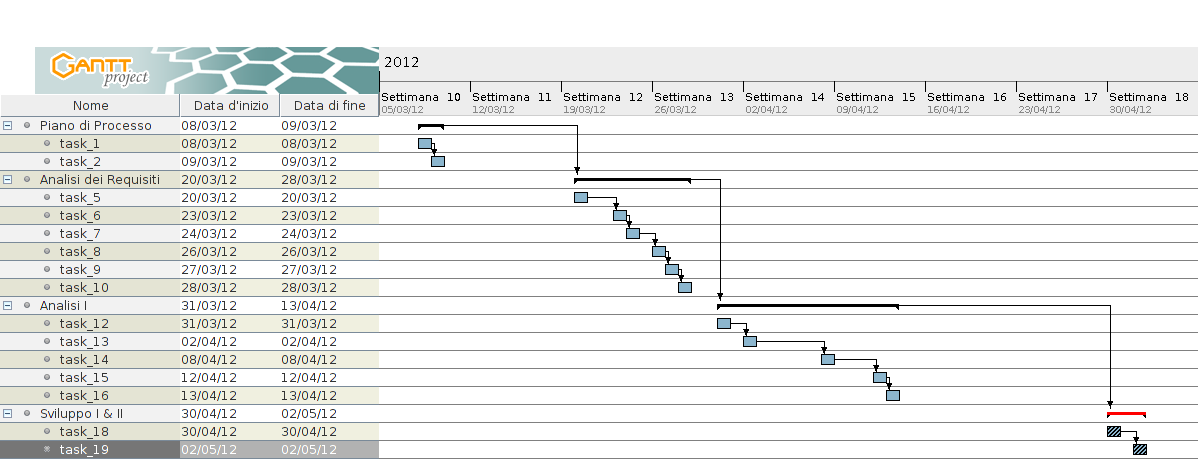
\includegraphics[scale=0.4]{lastdiagrs/gantt.png}
\caption{\textit{Developing's Gannt Diagram}.}
\label{fig:gannt}
\end{figure}
Possiamo ora rappresentare tutte le fasi dello sviluppo tramite il Diagramma di
Gannt proposto in Figura \vref{fig:gannt}.

\subsection{Testing}
Noi abbiamo effettuato due tipologie di testing: quello \textbf{white box} in 
allegato assieme al codice sorgente, e quello \textbf{black box}, che viene fornito
qui sotto.

\begin{description}
\item[Utente]

Identifichiamo i test lato utente

\begin{itemize}
 \diam \textit{Registrazione}
 
  Forniamo di seguito una descrizione dei passi da effettuare.
  \begin{description}
  
  \item[inserimento dei dati personali] Si ha input non valido qualora
  \begin{itemize}
  \item manca uno o più di un dato richiesto
  \item il codice fiscale contiene meno di 16 caratteri
  \item l'email è \textit{well-formed}
  \item la data non può contenere caratteri
  \end{itemize}
  \item[Invio di informazioni]
  \end{description}
  Si ha \textbf{successo} quando si ottiene un messaggio di conferma di effettuato
  inserimento dell'utente, e quindi si considera passato il test. Si ha invece
  \textbf{fallimento} qualora l'utente non sia stato inserito.


 \diam \textit{Accesso}

  È necessario effettuare l'inserimento delle credenziali per l'autenticazione,
  e conseguentemente effettuare il login.
  
  Si ha \textbf{successo} qualora l'utente utente riesca ad entrare nel sistema, 
  altrimenti si ha \textbf{fallimento} se l'utente non riesce ad autenticarsi, a causa
  di un'errata o mancata registrazione.                                      

 \diam \textit{Richiedere prenotazione}

  È opportuno inserire i dati, quali la scelta reparto
  e l'inserimento della descrizione dei ``sintomi'': in seguito bisogna
  inoltrare la richiesta. 
  
   L'esecuzione è avvenuta con \textbf{successo} se:
   \begin{itemize}
   \item si visualizza un messaggio di conferma
   \item il test di ``visualizzare delle prenotazioni'' è esso stesso riuscito.
   \end{itemize}
  altrimenti porta a \textbf{fallimento} se:
  \begin{itemize}
  \item l'utente non riesce ad inviare richiesta
  \item la visualizzione delle prenotazioni fallisce
  \end{itemize}
                                                                                                                                   

 \diam \textit{Visualizzare prenotazioni}


  Le prenotazioni vengono aggiornate tramite il comando di refresh. Se non 
  venissero visualizzate, allora si avrebbe un caso di fallimento. Altri possibili
  motivi di errore potrebbero essere i seguenti:
  \begin{itemize}
  \item si visualizzano le prenotazioni che appartengono ad un altro paziente
  \item si visualizzano delle prenotazioni che non sono state richieste
  \end{itemize}                                                                                                           

 \diam \textit{Posticipo prenotazione}


  Si effettua una scelta della prenotazione
  ed una richiesta di posticipazione


  In caso di \textbf{successo} si visualizza un messaggio di conferma, e si deve controllare
  successivamente alla gestione che la prenotazione sia stata effettivamente 
  posticipata. Si ha \textbf{fallimento} invece se:
  \begin{itemize}
  \item l'utente non riesce a fare la richiesta
  \item non si riesce a scegliere la prenotazione
  \item la prenotazione non viene posticipata
  \end{itemize}
                                                                                                                        

 \diam \textit{Cancellazione di prenotazione}


   Si effettua una scelta della prenotazione
  ed una richiesta di cancellazione

  In caso di \textbf{successo} si visualizza un messaggio di conferma, e si deve controllare
  successivamente alla gestione che la prenotazione sia stata effettivamente 
  cancellata. Si ha \textbf{fallimento} invece se:
  
  \begin{itemize} 
  \item non si riesce a fare la richiesta
  \item non si riesce a scegliere la prenotazione
  \item la prenotazione non viene cancellata
  \end{itemize}

                                                                                                                                   

 \diam \textit{Visualizzare referto}


  Si sceglie la  prenotazione di cui si vuole visualizzare referto, che deve
  essere visualizzata in caso di \textbf{successo}. In caso contrario, si ha il
  fallimento: altro caso di errata gestioen della visualizzazione è la visualizzazione
  del referto errato.

                                                                                                                                   

 \diam \textit{Logout}

 Avviene semplicemente uscendo dal programma: non dovrebbero essere previsti
 particolari casi di errore.
\end{itemize}

                                                                                                                                   
                                                                                                                                   
                                                                                                                                   

\item[Admin]

Identifichiamo i test lato amministratore.

                                                                                                                                   
\begin{itemize}
\diam \textit{Accesso}

  Come sopra

                                                                                                                                   

\diam \textit{Visualizzare le richieste(prenotazione, posticipazione, cancellazione)}

  Si ha \textbf{successo} se le richieste vengono visualizzate, altrimenti si ha
  \textbf{fallimento}
                                                                                                                                   

\diam \textit{Creare nuova prenotazione}

  Forniamo di seguito una descrizione dei passi da effettuare.
  \begin{description}
  \item scegliere richiesta da gestire;
  \item creare prenotazione: in particolare è necessario scegliere la data,
                        associare la stanza,
                        associare il medico
                        associare la priorità e
                        specificare il paziente;

  \item salva prentoazione
  \end{description}
  
  Si ha \textbf{successo} solo se la prenotazione è stata creata o salvata all'interno
  del database; in caso di \textbf{fallimento} invece, si potrebbero verificare i
  seguenti casi:
  \begin{itemize}
  \item la prenotazione non viene salvata
  \item non si riesce a scegliere la richiesta da gestire
  \item non si riescono ad editare data/stanza/medico/priorità.
  \end{itemize}

                                                                                                                                   

\diam \textit{Modificare prenotazione visualizzata}

  Forniamo qui la descrizione dei passi da effettuare.
  \begin{itemize}
  \item visualizzare le prenotazioni
  \item scegliere la prenotazione
  \item modificare della prenotazione
  \item salvare prenotazione
  \end{itemize}
  
  Si rientra nel caso di \textbf{successo} se la prenotazione è stata modificata e 
  salvata, altrimenti si potrebbero verificare i seguenti casi di fallimento:
  \begin{itemize} 
  \item le prenotazioni non vengono visualizzate
  \item non si riesce a scegliere la prenotazione
  \item l'edit fallisce
  \item le modifiche non vengono salvate    
  \end{itemize}   

                                                                                                                                   

\diam \textit{Posticipare prenotazione visualizzate}

  È necessario scegliere la prenotazione da posticipare, per poi inviare il comando
  di posticipa.
  
  L'operazione è stata effettuata con \textbf{successo} se la prenotazione viene
  effettivamente posticipata, altrimenti potrebbero avvenire i seguenti casi di
  errore:
  \begin{itemize}
  \item non si riesce a scegliere la prenotazione da posticipare
  \item la prenotazione non viene posticipata
  \item si riesce ad anticipare la prenotazione
  \end{itemize}

                                                                                                                                   

\diam \textit{Cancellare prenotazione visualizzata}


  È opportuno scegliere la prenotazione da cancellare, per poi inoltrare il 
  comando di cancellazione.


  Si ha \textbf{successo} se la prenotazione è stata opportunamente cancellata, altrimenti
  (in caso di \textbf{fallimento}) non si riesce a scegliere prenotazione da cancellare o/e
  la prenotazione non viene cancellata.

                                                                                                                                   
  
\diam \textit{Creare/modificare ed associare referti}

  È opportuno eseguire i seguenti step:
  \begin{itemize}
  \item scegliere la prenotazione da modificare
  \item creare o scegliere il referto da modificare
  \item associare referto
  \end{itemize}

  L'esecuzione è avvenuta con \textbf{successo} se il referto viene creato/modificato,
  altrimenti porta a \textbf{fallimento} se si verifica uno o più dei casi seguenti:
  \begin{itemize}
  \item failure - non si riesce a creare referto
  \item non si riesce ad associare referto
  \item si riesce ad associare piu di un referto alla stessa prenotazione
  \end{itemize}

                                                                                                                                   

\diam \textit{Visualizzare referti}

  
  È necessario scegliere la prenotazione di cui si vuole visualizzare referto.

  Si ha \textbf{successo} se il referto viene visualizzato, altrimenti in caso di
  \textbf{fallimento}  non viene visualizzato, o comunque non viene visualizzato il 
  referto previsto.
\end{itemize}
\end{description}

\subsection{Revisione dello sforzo del progetto}
Per effettuare una stima finale dello sforzo compiuto, ci basiamo sulle 
effettive righe di codice, calcolate tramite il tool \textsc{SLOCCount}
di \textit{David A. Wheeler}. Il nostro codice è costituito da $4642$ linee di codice,
con una stima molto prossima alle $4300$ precedentemente stimate (v. Sezione
\vref{sec:mfsvds}). Si ha inoltre un costo di produzione stimato di $\d 135.420$,
considerando un salario annuale medio di $\d 56.286$ per sviluppatore. 
Conseguentemente,  utilizzando sempre la formula di \textit{Bailey-Basili} per 
la valutazione dello sforzo, otterremo il seguente sforzo:
\[E_{bb} = 5.5 + 0.7 \cdot KLOC^{1,16}\simeq 9.65 mesi/persona\]

Effettuando la somma delle ore ottenute nel diario, otteniamo un totale di $111$ 
ore complessive di lavoro per ogni componente del gruppo. Stimando ora che ogni
componente del gruppo abbia lavorato per $5$ ore al giorno, dati che questo
team sta lavorando correntemente ad altri progetti, otteniamo un lavoro di $22$
giorni/persona continuativi. Possiamo comunque evidenziare come la stima ottenuta
tramite analisi dei FP, sia stata comunque una sovrastima del tempo che è stato
effettivamente necessario allo sviluppo. 


\subsection{Analisi di qualità}
\begin{figure}[!thp]
	\centering
	\subfloat[][\emph{Ciclomatic Complexity in Methods}.]{\label{subfig:ciclocomplxmet}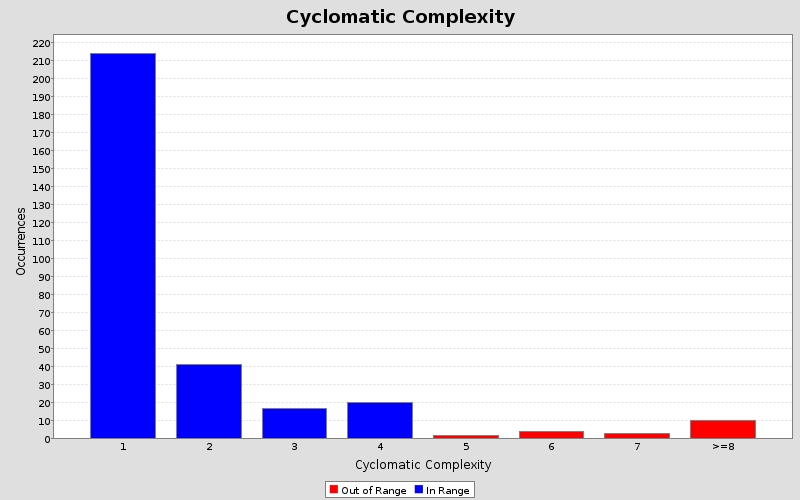
\includegraphics[scale=0.5]{lastdiagrs/CyclomaticComplexity_method.jpg}}\\
	\subfloat[][\emph{Number of Parameters in Methods}.]{\label{subfig:numparameter}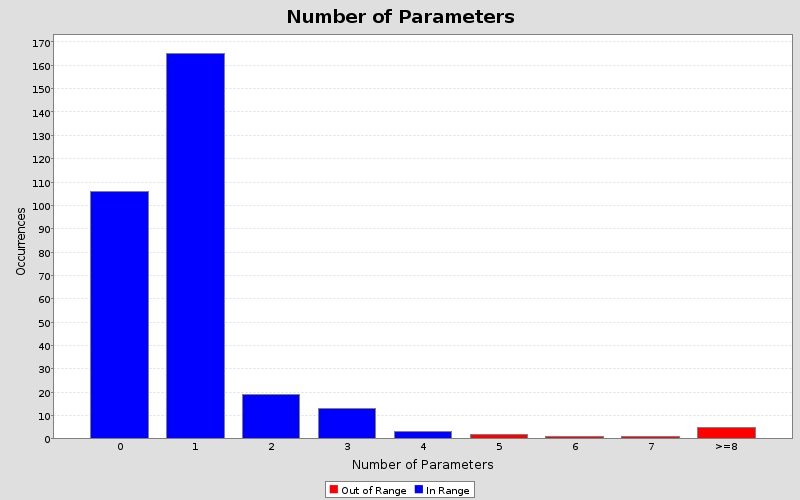
\includegraphics[scale=0.5]{lastdiagrs/NumberOfParameters_method.jpg}}\\
	\caption{\textit{Quality's Metrics (1)}.}
	\label{fig:qualmetrione}
\end{figure}
Tramite il tool \textsc{Metrics} di \textsc{Eclipse}, possiamo desumere le seguenti
considerazioni della qualità del software:
\begin{description}
\item[Complessità Ciclomatica] In Figura \vref{fig:qualmetrione}\subref{subfig:ciclocomplxmet},
	possiamo notare che sono pochi i metodi a possedere complessità ciclomatica
	alta: questi sono prevalentemente per la gestione della GUI, che comunque
	rimane al di sotto del limite $50$ di testabilità (Il massimo è raggiunto
	con \texttt{ClientUI} che ha Complessità Ciclomatica $26$).
\item[Numero di parametri] In figura \vref{fig:qualmetrione}\subref{subfig:ciclocomplxmet},
	Possiamo notare anche in questo caso che sono pochi i metodi nei quali
	si ha un elevato numero di parametri (il massimo raggiunto è 9): questo
	è dovuto al fatto che spesso la creazione di istanze di oggetti per 
	record del database, necessiti esso stesso un numero di parametri pari
	agli attributi delle tabelle nel suddetto database.
\begin{figure}
\centering
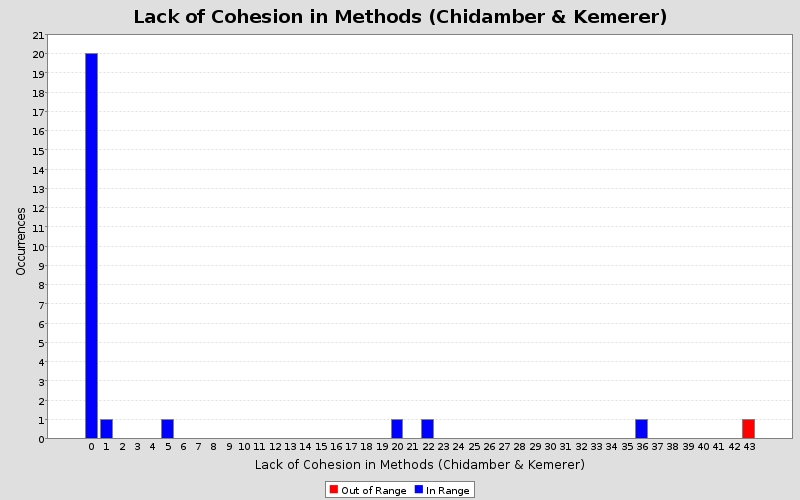
\includegraphics[scale=0.5]{lastdiagrs/ackOfCohesionInMethods_chidamberKemerer}
\caption{\textit{Quality's Metrics (2) - Mancanza di Coesione nei Metodi}.}
\label{fig:qomlackcohesion}
\end{figure}
\item[Mancanza di Coesione nei Metodi] Abbiamo considerato queste stime, anche
	se sono considerate poco attendibili dallo stesso tool di sviluppo
	\footnote{«Despite its importance, it is difficult to establish a clear 
	mechanism for measuring it. This is probably due to the fact that good 
	abstractions have deep semantics and a class that is clearly cohesive 
	when viewed from a semantic point of view may not be so when viewed from
	 a purely symbolic point of view.

	As an aside, the somewhat inelegant name is due to the wish to have lower
	 metric values representing a 'better' situation.» 
	 
	 \texttt{http://eclipse-metrics.sourceforge.net/descriptions/pages/cohesion/\\
	 LackOfCohesionInMethods.html}}.
	Utilizzando la stima di \textit{Chidamber-Kemerer}, possiamo evidenziare
	che l'unica classe che risulti problematica sia quella \textsc{Paziente}:
	tuttavia ci teniamo a sottolineare che gran parte del codice con Mancanza
	di Coesione è in gran parte generato automaticamente dal plug-in di 
	\textsc{Eclipse} per la creazione di GUI, e che quindi è difficilmente
	rifattorizzabile, a costo di introdurre ulteriori errori (v. Figura 
	\vref{fig:qomlackcohesion}).
\end{description}


\subsection{Valutazione del ruolo produttivo}
In questo punto forniamo una descrizione della valutazione personale del ruolo
produttivo da noi ricoperto.
\begin{description}
\item[Bergami Giacomo] In quanto \textit{Quality Manager} del team, posso sottolineare
	come sia stato periglioso la gestione della documentaizone, in quanto
	dovevo garantire l'omogeneità del documento finale, e indicare i punti
	della documentazione che non erano stati svolti in modo corretto.
	
	Per quanto concerne invece la generazione dei test, il mio compito è
	stato delegato a Fabian Priftaj per il \textit{white box}, in quanto conosceva
	maggiormente il codice, ed a Matej Torok per il \textit{black box}, per
	l'esperienza avuta sul campo con progetti precedenti.
\item[De Luca Paolo] Le responsabilità dovute alla carica di \textit{Tool specialist}, si
	sono riversate anche sul resto del team, in quanto ci è stato necessario
	usare molti di strumenti nuovi, senza alcuna esperienza 
	precedente. In questo quadro, la scelta degli strumenti si è spesso 
	riversata verso strumenti quanto più semplici da utilizzare e facilmente
	accessibili.

	Tuttavia, l'utilizzo di \textsc{ArgoUML} è stato spesso stressante a causa 
	dell'instabilità e la ridotta usabilita dello stesso. Altra nota di 
	demerito va ad \textsc{Eclipse}, poichè la generazione di una semplice 
	interfaccia grafica richiede molto tempo ma soprattutto un hardware 
	molto prestante, anche per semplici oggetti: infatti è necessario attendere
	un delay molto elevato per ogni aggiunta/modifica all'interfaccia.
\item[Fabian Priftaj] [TODO -DEVELOPER]
\item[Torok Matej] [TODO -SUPERVISOR]
\end{description}

Come ultima osservazione, possiamo affermare che con questo progetto abbiamo 
potuto apprezzare l'utilizzo di tool automatici per l'ottenimento di risultati
efficaci in tempi immediati: faccio riferimento soprattuto agli ultimi Diagrammi
di Interazione ed alla valutazione della qualità, che prevede dei calcoli lunghi
e laboriosi nei metodi delle classi.

Da questo progetto abbiamo imparato che, allo scopo di scrivere una documentaizone
completa e dettagliata, è necessario impiegare molto tempo: questo può essere
tuttavia svantaggioso qualora i possibili \textit{competitor} impieghino meno 
energie nella sua produzione, allo scopo di produrre il prodotto finale il 
prima possibile al cliente. 

Siamo consapevoli che il progetto consegnato sarebbe stato ulteriormente migliorabile,
ad esempio tenendo conto dell'efficienza e della responsività; avremmo potuto
rendere inoltre il codice maggiormente riusabile, inserendo un ulteriore 
\textit{layer} software tra l'interfaccia grafica e database, applicando eventualmente
altri design pattern per gestire quest'ulteriore livello di indirezione, utilizzando
ad esempio l'\textit{Hollywood Principle}.
